\begin{frame}
  \frametitle{Heart Modeling}
  \begin{itemize}
  \item modeling \emph{pathologies}: e.g. ischemic heart
  \item parameter identification from displacements, pressure measurements
  \item output: \emph{global indicators} of beating heart: blood pressure,
    ejection volume
  \item in collaboration with INRIA Rocquencourt, France (Jacques Sainte-Marie,
    Dominique Chapelle and others)
  \end{itemize}
  \begin{center}
    \begin{minipage}{0.28\linewidth}
      \scriptsize
      action potential \\
      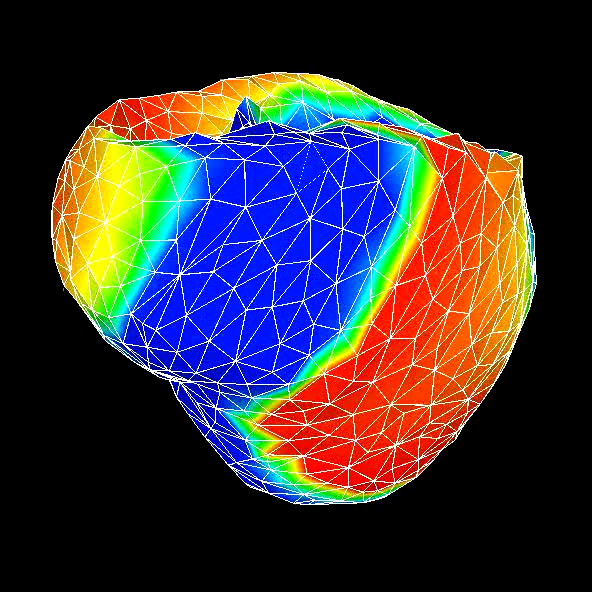
\includegraphics[width=0.9\linewidth]{\figDirMacroHeart/activ1}
    \end{minipage}
    \hfill
    \begin{minipage}{0.4\linewidth}
      \scriptsize
      global indicators: healthy (dashed) and ischemic (solid) heart \\
      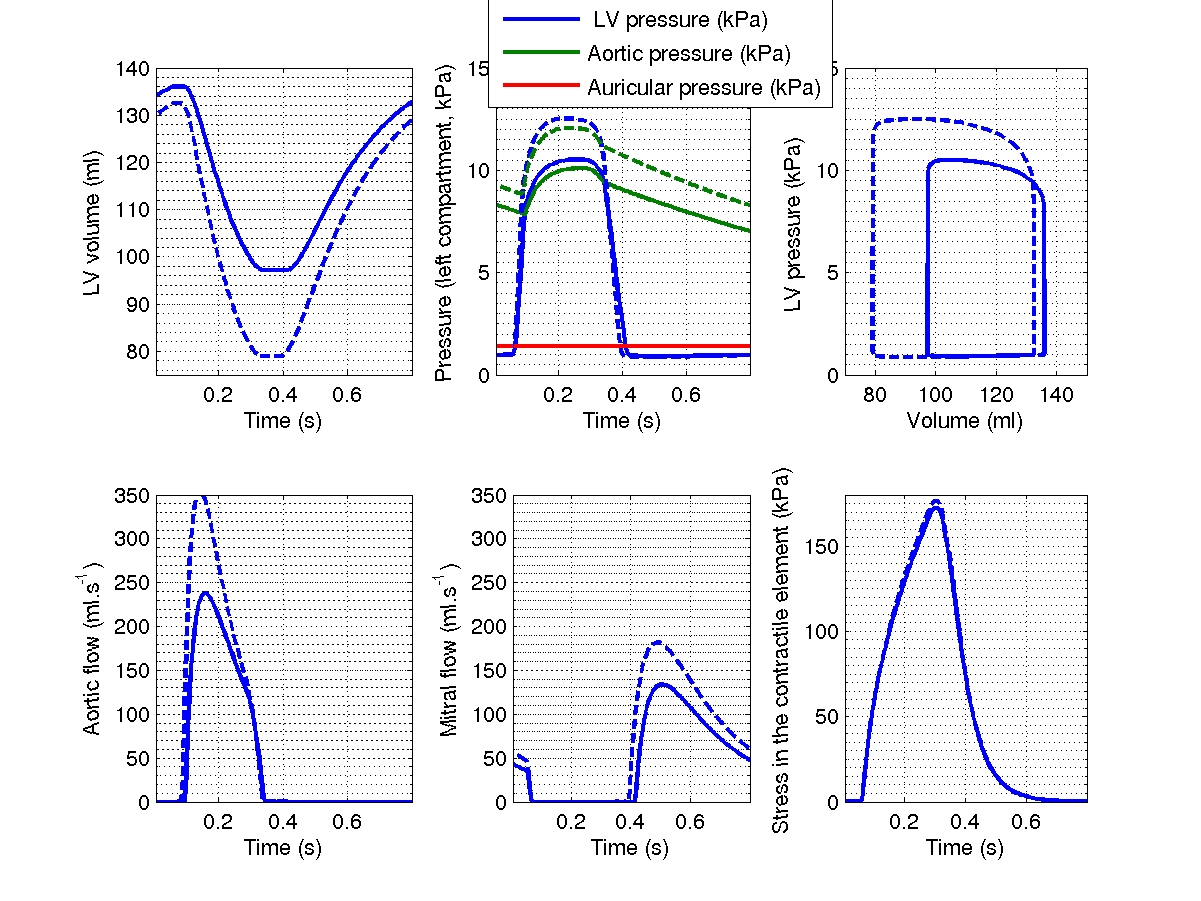
\includegraphics[width=\linewidth]{\figDirMacroHeart/compar_u1}
    \end{minipage}
    \hfill
    \begin{minipage}{0.28\linewidth}
      \scriptsize
      stress in ischemic heart \\
      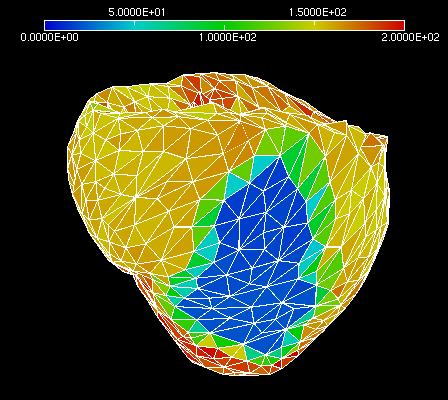
\includegraphics[width=0.9\linewidth]{\figDirMacroHeart/stress_path}
    \end{minipage}
  \end{center}
\end{frame}
